\documentclass[11pt]{amsart}
\usepackage[margin=1.05in]{geometry}
\usepackage{amsmath,amssymb,amsthm,mathtools}
\usepackage{booktabs,array}
\usepackage[shortlabels]{enumitem}
\usepackage{listings}
\usepackage{tikz}
\usepackage[hidelinks]{hyperref}
\hypersetup{pdftitle={A bag reduction for the Randic-radius problem}}

\lstset{basicstyle=\ttfamily\scriptsize,columns=fullflexible,breaklines=true,frame=single,
        showstringspaces=false,keepspaces=true}

\newtheorem{theorem}{Theorem}[section]
\newtheorem{lemma}[theorem]{Lemma}
\newtheorem{proposition}[theorem]{Proposition}
\newtheorem{corollary}[theorem]{Corollary}
\newtheorem{conjecture}[theorem]{Conjecture}
\newtheorem{introthm}{Theorem}
\renewcommand{\theintrothm}{\Alph{introthm}}
\theoremstyle{definition}
\newtheorem{definition}[theorem]{Definition}
\newtheorem{remark}[theorem]{Remark}

\DeclareMathOperator{\rad}{rad}
\DeclareMathOperator{\diam}{diam}
\DeclareMathOperator{\ecc}{ecc}
\newcommand{\Rp}{R'}
\newcommand{\C}{\mathcal{C}}
\newcommand{\kmax}{11}
\newcommand{\mumax}{5}

\begin{document}

\title[A bag reduction for the Randi\'c--radius problem]{A bag reduction for the Randi\'c--radius problem:\\
graphs with small two-edge-connected components,\\ and exhaustive verification through eleven vertices}

\author{Anonymous}
\date{October 2026}

\begin{abstract}
For a graph $G$ let $R(G)=\sum_{uv\in E(G)}(d_ud_v)^{-1/2}$ be the Randi\'c index and
$\Rp(G)=\sum_{uv\in E(G)}1/\max(d_u,d_v)$ its modified version; always $R\ge \Rp$.
Fajtlowicz's conjecture (1988) asserts $R(G)\ge\rad(G)-1$ for every connected graph, and
Caporossi and Hansen (2000) conjectured $R(G)\ge\rad(G)$ for every connected graph other than a path on an
even number of vertices. \emph{Both conjectures remain open; this paper does not prove either of them.}
We study the stronger inequality $\Rp(G)\ge\rad(G)-\tfrac12$, proved for chemical graphs by Cygan,
Pilipczuk and \v{S}krekovski. Our results are the following.
(i) In every class of graphs closed under connected subgraphs and under replacing a shallow branch behind a
bridge by a path, a counterexample with the fewest vertices (and then edges) consists of one bridgeless core with pendant paths,
and the associated \emph{bag} violates the inequality $\Rp(H)\ge\rad(C(H))+1$ of Cygan, Pilipczuk and \v{S}krekovski.
(ii) An exhaustive computation in exact arithmetic shows that this bag inequality holds for every bag whose core
has at most $\kmax$ vertices.
(iii) Consequently $\Rp(G)\ge\rad(G)-\tfrac12$, and hence Fajtlowicz's bound, holds for every connected graph
each of whose two-edge-connected components has at most $\kmax$ vertices, or cyclomatic number at most $\mumax$, or only vertices of degree at most four.
(iv) We prove an exact conservation identity for supportive edges and derive from it an antichain inequality.
(v) We verify (in exact arithmetic for $\Rp$, and with rigorous floating-point error control for $R$) that all
$1{,}018{,}690{,}328$ connected graphs with $2\le n\le 11$ vertices satisfy
$\Rp\ge\rad-\tfrac12$, that those with at most one vertex of degree one satisfy $\Rp\ge\rad$, and that the
Caporossi--Hansen inequality holds for all of them, with equality exactly for $K_2,C_4,C_6,C_8,C_{10}$.
All programs are reproduced in the appendix.
\end{abstract}

\maketitle

\section{Introduction}

All graphs are finite and simple. For a connected graph $G$ and a vertex $v$ we write $d_v$ for the degree,
$\ecc(v)=\max_w d(v,w)$ for the eccentricity, $\rad(G)=\min_v\ecc(v)$, $\diam(G)=\max_v\ecc(v)$ and
$\mu(G)=|E(G)|-|V(G)|+1$ for the cyclomatic number. The Randi\'c index~\cite{Randic} and the modified
Randi\'c index of Dvo\v{r}\'ak, Lidick\'y and \v{S}krekovski~\cite{DLS} are
\[
R(G)=\sum_{uv\in E(G)}\frac1{\sqrt{d_ud_v}},\qquad \Rp(G)=\sum_{uv\in E(G)}\frac1{\max(d_u,d_v)} .
\]
Since $\sqrt{d_ud_v}\le\max(d_u,d_v)$, we have $R(G)\ge \Rp(G)$, with equality exactly when every component is regular.

\begin{conjecture}[Fajtlowicz~\cite{Fajtlowicz}]\label{conj:F}
Every connected graph $G$ satisfies $R(G)\ge\rad(G)-1$.
\end{conjecture}

\begin{conjecture}[Caporossi and Hansen~\cite{CaporossiHansen}]\label{conj:CH}
Every connected graph $G$ that is not a path on an even number $n\ge4$ of vertices satisfies $R(G)\ge\rad(G)$.
\end{conjecture}

The even paths must be excluded, since $R(P_{2k})=k-\tfrac32+\sqrt2<k=\rad(P_{2k})$ for $k\ge2$.

\subsection*{Known results}
For trees, Caporossi and Hansen proved $R(T)\ge\rad(T)+\sqrt2-\frac32$~\cite{CaporossiHansen}, and Deng, Tang and Zhang
proved $R(T)>\rad(T)+\frac1{15}$ for every tree other than an even path~\cite{DTZ}, which settles
Conjecture~\ref{conj:CH} for trees. Dvo\v{r}\'ak, Lidick\'y and \v{S}krekovski~\cite{DLS} proved $\Rp(G)\ge\diam(G)/2$ for every connected graph,
which gives $R(G)\ge\rad(G)/2$; Yang and Lu~\cite{YangLu} proved the sharp bound $R(G)-\diam(G)/2\ge\sqrt2-1$ for
$n\ge3$. Cygan, Pilipczuk and \v{S}krekovski~\cite{CPS} proved $\Rp(G)\ge\rad(G)-\tfrac12$ for every connected graph
of maximum degree at most four, and Conjecture~\ref{conj:CH} for such graphs. Deng, Tang and Zhang~\cite{DTZ}
proved $R(G)\ge\rad(G)-\tfrac{31}{105}(\mu(G)-1)$ when $\mu(G)\ge1$; this settles Conjecture~\ref{conj:F} for
$\mu\le4$. Doig~\cite{Doig1,Doig2} verified Conjecture~\ref{conj:CH} for cacti. Further special classes were treated
by You and Liu~\cite{YouLiu} and others; see~\cite{DLS}. An unrefereed manuscript in a public corpus~\cite{Corpus054}
develops a structure theory for minimal counterexamples to Conjecture~\ref{conj:CH} (supportive edges, radius-stable
peeling, rooted Yang--Lu replacement) and reports a computer verification for $\mu\le 8$; Section~\ref{sec:structure}
adapts that approach to $\Rp$. As far as we know, Conjectures~\ref{conj:F} and~\ref{conj:CH} are open in general.

\subsection*{The inequality studied here}
We work with the modified index and the inequality
\begin{equation}\label{A}\tag{A}
\Rp(G)\ \ge\ \rad(G)-\tfrac12 \qquad\text{for every connected graph } G .
\end{equation}
Since $R\ge\Rp$, inequality \eqref{A} implies $R(G)\ge\rad(G)-\frac12$ and hence Conjecture~\ref{conj:F}.
It is sharp: $\Rp(P_{2k})=k-\tfrac12$. Cygan, Pilipczuk and \v{S}krekovski proved~\eqref{A} for maximum degree at
most four; the degree bound enters their proof only through an inequality for \emph{bags}
(Definition~\ref{def:bag}), and they remarked that this inequality for all bags would imply
Conjecture~\ref{conj:F}~\cite{CPS}. Inequality~\eqref{A} is open.

\subsection*{Results}
A class $\C$ of connected graphs is \emph{admissible} if it is closed under taking connected subgraphs and under the
pendant-path replacement of Lemma~\ref{lem:replace}. The class of all connected graphs is admissible.

\begin{introthm}[Theorems~\ref{thm:structure} and~\ref{thm:bagred}]\label{introA}
Let $\C$ be admissible and let $G\in\C$ violate~\eqref{A}, with $|V(G)|$ minimal and then $|E(G)|$ minimal.
Then the $2$-core $K$ of $G$ is bridgeless, $G$ is $K$ together with pendant paths, every vertex of $K$ carries at
most one of them, at most one has length $\ge2$, and $|V(K)|\le2\mu(G)+1$. The graph $H$ obtained by
shortening every pendant path to a single edge is a bag with core $K$, and $\Rp(H)<\rad(K)+1$.
\end{introthm}

\begin{introthm}[Theorem~\ref{thm:bagcomp}]\label{introB}
Every bag $H$ whose core has at most $\kmax$ vertices satisfies $\Rp(H)\ge\rad(C(H))+1$. Equality holds only for
$K_{2,3}$ with one pendant vertex attached to each of its five vertices.
\end{introthm}

\begin{introthm}[Theorem~\ref{thm:main}]\label{introC}
Let $G$ be a connected graph such that every two-edge-connected component $B$ of $G$ satisfies
$|V(B)|\le\kmax$, or $\mu(B)\le\mumax$, or $d_G(v)\le4$ for all $v\in V(B)$. Then $\Rp(G)\ge\rad(G)-\frac12$. In
particular $R(G)\ge\rad(G)-\frac12$, so Conjecture~\ref{conj:F} holds for $G$.
\end{introthm}

The class in Theorem~\ref{introC} contains, for example, all graphs obtained by joining arbitrarily many graphs of
order at most $\kmax$ by bridges, and attaching arbitrary trees; such graphs can have unbounded cyclomatic number and
unbounded maximum degree. For cyclomatic number at most four and for chemical graphs the conclusion for $R$ was
known~\cite{DTZ,CPS}; the unrefereed manuscript~\cite{Corpus054} reports Conjecture~\ref{conj:CH} for cyclomatic number at
most eight.

\begin{introthm}[Theorem~\ref{thm:conservation} and Theorem~\ref{thm:antichain}]\label{introD}
Let $Q$ be a set of vertices all of whose outside neighbours have smaller degree. Then the total ``injection''
$\sum_{v\in Q}p_v\,b_v$ through the edges leaving $Q$ equals the total slack of the strict edges inside $Q$ plus an
explicit nonnegative term carried by equal-degree edges. If the strict edges inside $Q$ are supportive, every antichain of
the degree order in $Q$ has weight at most the injection below it.
\end{introthm}

\begin{introthm}[Theorem~\ref{thm:exhaustive}]\label{introE}
Every connected graph on at most $11$ vertices satisfies~\eqref{A}. Every such graph with at most one vertex of degree
one satisfies $\Rp(G)\ge\rad(G)$. Every such graph that is not an even path on at least four vertices satisfies
$R(G)\ge\rad(G)$, with equality exactly for $K_2$, $C_4$, $C_6$, $C_8$, $C_{10}$.
\end{introthm}

\subsection*{Relation to earlier work}
Theorem~\ref{introA} combines three ingredients: the bag concept and the inequality~\eqref{B} of Cygan, Pilipczuk and
\v{S}krekovski~\cite{CPS}; the reduction tools for minimal counterexamples (supportive edges, peeling, rooted replacement)
that the manuscript~\cite{Corpus054} develops for $R$ and Conjecture~\ref{conj:CH}; and the bound of
Theorem~\ref{thm:DLS}. Working with $\Rp$ instead of $R$ makes every identity rational, so that all computations are exact,
and the reduction ends in an inequality that involves only the core and its pendant vertices. This is what allows a
certification core by core,
independently of the cyclomatic number of the whole graph (Theorem~\ref{introC}), whereas~\cite{Corpus054} bounds the
order of the core through the cyclomatic number. Theorem~\ref{introD} and the exhaustive verification for $n=11$ are new as
far as we know.

\subsection*{What is not proved}
We do not prove Conjecture~\ref{conj:F}, Conjecture~\ref{conj:CH}, or inequality~\eqref{A} in general. By
Theorem~\ref{introA}, inequality~\eqref{A} for all graphs would follow from the bag inequality for all bags
(Conjecture~\ref{conj:bag}); we verify that inequality only for cores of order at most~$\kmax$. Section~\ref{sec:open}
lists the remaining gap and further conjectures, together with the evidence for them.

\section{Preliminaries}\label{sec:prelim}

Let $G$ be a graph. For a vertex $v$ with $d_v\ge2$ put
\[
\lambda_v=|\{w\in N(v):d_w<d_v\}|,\quad h_v=d_v-\lambda_v,\quad g_v=d_v(d_v-1),\quad
a_v=\frac{\lambda_v}{g_v},\quad b_v=\frac{h_v}{g_v}.
\]
Thus $\lambda_v$ counts the \emph{lower} neighbours of $v$, $h_v$ counts the neighbours of degree at least $d_v$,
and $a_v+b_v=\frac1{d_v-1}$. A vertex with $\lambda_v=0$ is \emph{locally minimal}. A vertex of degree one is a
\emph{leaf}, and its neighbour is its \emph{support}. An edge $e$ is \emph{supportive} if $\Rp(G-e)>\Rp(G)$.

\begin{lemma}[Edge deletion]\label{lem:edge}
Let $uv\in E(G)$ with $d_u,d_v\ge2$, and let $\beta_u$ be the number of neighbours $w\neq v$ of $u$ with $d_w<d_u$
(and symmetrically $\beta_v$). Then
\[
\Rp(G-uv)-\Rp(G)=-\frac1{\max(d_u,d_v)}+\frac{\beta_u}{g_u}+\frac{\beta_v}{g_v}.
\]
In particular:
\begin{enumerate}[(i)]
\item if $d_u<d_v$, then $\Rp(G-uv)-\Rp(G)=a_u-b_v$, so $uv$ is supportive if and only if $a_u>b_v$;
\item if $d_u=d_v=k$, then $\Rp(G-uv)-\Rp(G)=\frac{\lambda_u+\lambda_v}{k(k-1)}-\frac1k$, so $uv$ is supportive if and
only if $\lambda_u+\lambda_v\ge k$.
\end{enumerate}
\end{lemma}

\begin{proof}
Only the terms of edges at $u$ or $v$ change. The term of $uv$ disappears. For $w\in N(u)\setminus\{v\}$ the term
$1/\max(d_u,d_w)$ becomes $1/\max(d_u-1,d_w)$: it is unchanged if $d_w\ge d_u$, and it increases from $1/d_u$ to
$1/(d_u-1)$, that is by $1/g_u$, if $d_w<d_u$. The same holds at $v$. This proves the formula. If $d_u<d_v$ then
$\beta_u=\lambda_u$ and $\beta_v=\lambda_v-1$, and $-\frac1{d_v}+\frac{\lambda_v-1}{g_v}=-\frac{d_v-\lambda_v}{g_v}=-b_v$.
If $d_u=d_v=k$ then $\beta_u=\lambda_u$, $\beta_v=\lambda_v$, and the expression is positive iff
$\lambda_u+\lambda_v>k-1$.
\end{proof}

\begin{lemma}[Locally minimal vertices]\label{lem:locmin}
If $d_u\ge2$ and $\lambda_u=0$, then no edge at $u$ is supportive.
\end{lemma}

\begin{proof}
Let $uv$ be an edge. As $u$ has no lower neighbour, $d_v\ge d_u$. If $d_v>d_u$, Lemma~\ref{lem:edge}(i) gives
$\Rp(G-uv)-\Rp(G)=a_u-b_v=-b_v\le0$. If $d_v=d_u=k$, then $\lambda_v\le k-1$ because $u$ is not lower than $v$, and
Lemma~\ref{lem:edge}(ii) gives $\frac{\lambda_v}{k(k-1)}-\frac1k\le0$.
\end{proof}

\begin{lemma}[Deleting leaves]\label{lem:leaves}
Let $L$ be a set of leaves of $G$ with pairwise distinct supports, let $S$ be the set of these supports, and assume
$d_s\ge2$ for $s\in S$. Then, with all quantities computed in $G$,
\[
\Rp(G)-\Rp(G-L)=\sum_{s\in S}b_s-\sum_{\substack{st\in E(G),\ s,t\in S\\ d_s=d_t}}\frac1{g_s}\ \ge 0 .
\]
In particular $\Rp(G)-\Rp(G-\ell)=b_s\ge0$ for a single leaf $\ell$ with support $s$.
\end{lemma}

\begin{proof}
Deleting $L$ lowers the degree of each $s\in S$ by one and changes no other degree. The leaf edge at $s$ contributes
$1/d_s$ and disappears. Consider an edge $sw$, $s\in S$, $w\notin L$. If $w\notin S$, its term increases by $1/g_s$
when $d_w<d_s$ and is unchanged otherwise. If $w\in S$, its term $1/\max(d_s,d_w)$ becomes
$1/\max(d_s-1,d_w-1)$; it increases by $1/g_s$ when $d_w<d_s$, by $1/g_w$ when $d_w>d_s$, and by $1/g_s$ when
$d_w=d_s$. Collecting, the total increase equals $\sum_{s\in S}(\lambda_s-1)/g_s$ plus one term $1/g_s$ for each
equal-degree edge inside $S$ (the leaf at $s$ is one of the $\lambda_s$ lower neighbours). Since
$\frac1{d_s}-\frac{\lambda_s-1}{g_s}=\frac{h_s}{g_s}=b_s$, the formula follows. For nonnegativity delete the
leaves one at a time; by the case $|L|=1$ each step lowers $\Rp$ by some $b\ge0$.
\end{proof}

\begin{lemma}[Peeling]\label{lem:peel}
Let $S\subset V(G)$ be such that $G-S$ is connected and every vertex of $S$ has a neighbour outside $S$. Then
$\rad(G-S)\ge\rad(G)-1$.
\end{lemma}

\begin{proof}
Let $c$ be a centre of $G-S$. Every vertex outside $S$ is within distance $\rad(G-S)$ of $c$ in $G-S$, hence in $G$,
and every vertex of $S$ is adjacent to such a vertex. So $\ecc_G(c)\le\rad(G-S)+1$.
\end{proof}

\begin{theorem}[Dvo\v{r}\'ak, Lidick\'y and \v{S}krekovski~\cite{DLS}]\label{thm:DLS}
Every connected graph $G$ satisfies $\Rp(G)\ge\diam(G)/2$.
\end{theorem}

For a connected graph $H$ and $y\in V(H)$ let $\Rp_{y}(H)$ denote the value of $\Rp(H)$ computed with the degree of $y$
replaced by $d_H(y)+1$ (as if $y$ had one more neighbour outside $H$).

\begin{lemma}[Rooted form of Theorem~\ref{thm:DLS}]\label{lem:rooted}
If $H$ is connected and $y\in V(H)$ has $\ecc_H(y)=e$, then $\Rp_y(H)\ge\frac{e+1}2-\frac1{d_H(y)+1}$.
\end{lemma}

\begin{proof}
Add a new vertex $z$ adjacent only to $y$. The new graph $H^+$ satisfies $\Rp(H^+)=\Rp_y(H)+\frac1{d_H(y)+1}$ and
$\diam(H^+)\ge\ecc_{H^+}(z)=e+1$. Apply Theorem~\ref{thm:DLS} to $H^+$.
\end{proof}

\begin{lemma}[Pendant-path replacement]\label{lem:replace}
Let $xy$ be a bridge of a connected graph $G$, let $G_x\ni x$ and $G_y\ni y$ be the components of $G-xy$, and put
$e_x=\ecc_{G_x}(x)$, $e_y=\ecc_{G_y}(y)$. Assume $e_y\le e_x$. Let $G'$ be obtained from $G_x$ by attaching at $x$ a
new path with $e_y+1$ edges. Then $\Rp(G')\le\Rp(G)$ and $\rad(G')\ge\rad(G)$. Moreover $|V(G')|\le|V(G)|$, with
equality if and only if $G_y$ is a path having $y$ as an end vertex.
\end{lemma}

\begin{proof}
If $G_y=\{y\}$ there is nothing to prove, so let $e_y\ge1$. The vertex $x$ has the same degree $d_x$ in $G$ and $G'$, so
the edges of $G_x$ contribute the same amount to $\Rp(G)$ and $\Rp(G')$. Put $d_y=d_G(y)\ge2$. The remaining
contributions are $\frac1{\max(d_x,d_y)}+\Rp_y(G_y)$ in $G$ and $\frac1{\max(d_x,2)}+\frac{e_y}2$ in $G'$ (all vertices
of the new path except its end have degree two). By Lemma~\ref{lem:rooted},
\[
\Rp(G)-\Rp(G')\ \ge\ \frac12+\frac1{\max(d_x,d_y)}-\frac1{d_y}-\frac1{\max(d_x,2)} .
\]
If $d_x\le d_y$ the right side is $\frac12-\frac1{\max(d_x,2)}\ge0$; if $d_x>d_y\ge2$ it is $\frac12-\frac1{d_y}\ge0$.

For the radius, a vertex $v\in V(G_x)$ has $\ecc_{G'}(v)=\max(\ecc_{G_x}(v),d(v,x)+1+e_y)=\ecc_G(v)$. A vertex of the
new path at distance $j\ge1$ from $x$ has eccentricity at least $j+e_x\ge1+e_x$ in $G'$, while
$\rad(G)\le\ecc_G(x)=\max(e_x,1+e_y)\le 1+e_x$. Hence $\rad(G')\ge\rad(G)$. Finally $|V(G_y)|\ge e_y+1$, with equality
exactly when $G_y$ is a path starting at $y$.
\end{proof}

\section{Minimal counterexamples}\label{sec:structure}

\begin{definition}
A class $\C$ of connected graphs is \emph{admissible} if (a) every connected subgraph of a member of $\C$ is in $\C$,
and (b) whenever $G\in\C$ and $xy$, $G_x$, $G_y$, $G'$ are as in Lemma~\ref{lem:replace}, also $G'\in\C$.
\end{definition}

\begin{theorem}[Structure]\label{thm:structure}
Let $\C$ be admissible and let $G\in\C$ violate~\eqref{A}, with $|V(G)|$ minimal and, subject to this, $|E(G)|$
minimal among such graphs in $\C$. Put $r=\rad(G)$ and let $K$ be the $2$-core of $G$. Then:
\begin{enumerate}[(a)]
\item $G$ is not a tree and $\diam(G)\le2r-2$;
\item every edge of $G$ lying on a cycle is supportive;
\item $K$ is connected and bridgeless, and $E(G)\setminus E(K)$ is the set of bridges of $G$;
\item every component of $G-E(K)$ with at least two vertices is a path that meets $K$ in exactly one vertex, which is
one of its ends (a \emph{pendant path}); every vertex of $K$ is an end of at most one pendant path; there is at least one
pendant path, and at most one of them has length at least two;
\item every vertex of $K$ has degree at least three in $G$ and is not locally minimal; every vertex whose degree in
$K$ is two or three carries a pendant path;
\item at most three vertices have degree two in $K$; consequently $|V(K)|\le2\mu(K)+1=2\mu(G)+1$;
\item for every leaf $\ell$ we have $\rad(G-\ell)=r-1$, and for every nonempty set $L$ of leaves
$\Rp(G)-\Rp(G-L)<1$.
\end{enumerate}
\end{theorem}

\begin{proof}
Throughout, every graph obtained from $G$ by the operations below lies in $\C$ by admissibility, and if it violates
\eqref{A} it contradicts the minimality of $G$.

\emph{(a)} If $\diam(G)\ge2r-1$, Theorem~\ref{thm:DLS} gives $\Rp(G)\ge r-\frac12$. A tree has $\diam\ge2\rad-1$.

\emph{(b)} Let $e$ lie on a cycle. Then $G-e$ is connected, has the same vertices and fewer edges, and
$\rad(G-e)\ge r$ because distances do not decrease. If $\Rp(G-e)\le\Rp(G)$ then $G-e$ violates~\eqref{A}.

\emph{Bridges.} Let $xy$ be a bridge with $e_y\le e_x$ (notation of Lemma~\ref{lem:replace}). If $G_y$ is not a path
starting at $y$, the graph $G'$ of Lemma~\ref{lem:replace} has fewer vertices, $\Rp(G')\le\Rp(G)<r-\frac12\le
\rad(G')-\frac12$, a contradiction. So: \emph{for every bridge, a side of smaller or equal eccentricity is a path
starting at the bridge}.

\emph{(c)} Since $G$ is not a tree, $K\neq\emptyset$; $K$ is connected, all cycles of $G$ lie in $K$, and the edges
outside $K$ are bridges. Suppose an edge $xy$ of $K$ is a bridge of $G$. On the side $G_x$, every vertex of $K$
other than $x$ keeps its $K$-degree (at least two), and $x$ keeps $K$-degree at least one; if $K\cap G_x$ were a
forest, it would be the single vertex $x$ (impossible, as $d_K(x)\ge2$) or would have two vertices of degree at most
one. So $G_x$ contains a cycle, and so does $G_y$. Then neither side is a path, contradicting the previous paragraph.
Hence $K$ is bridgeless and the bridges of $G$ are exactly the edges outside $K$.

\emph{(d), first part.} The components of $G-E(K)$ are trees, each meeting $K$ in one vertex. Let $wy$ be an edge
with $w\in V(K)$, $y\notin V(K)$. The side $G_w$ contains a cycle, so it is not a path; by the bridge statement
applied in both directions we get $e_y<e_w$ and that $G_y$ is a path starting at $y$. Hence every branch at a vertex of
$K$ is a pendant path, and a pendant path with $s$ edges attached at $w$ satisfies $s\le\ecc_{G_w}(w)$.

\emph{(g), first part.} Let $\ell$ be a leaf with support $s$. By Lemma~\ref{lem:leaves}, $\Rp(G-\ell)\le\Rp(G)$. If
$\rad(G-\ell)\ge r$, the graph $G-\ell$ violates~\eqref{A}. Hence $\rad(G-\ell)\le r-1$, and equality holds by
Lemma~\ref{lem:peel}. Choose $c$ with $\ecc_{G-\ell}(c)\le r-1$. Since $\ecc_G(c)\ge r$ and deleting a leaf does not
change the other distances, $d(c,\ell)=r$, and every other vertex is within distance $r-1$ of $c$.

\emph{(d), second part.} Suppose two leaves $\ell,\ell'$ have the same support $s$, and let $c$ be as above for $\ell$.
If $c\neq\ell'$, then $d(c,\ell')=d(c,s)+1=d(c,\ell)=r$, although $\ell'$ is a vertex of $G-\ell$; this is impossible.
If $c=\ell'$, then every vertex of $G-\ell$ is within distance $r-1=d(c,\ell)-1=1$ of the leaf $\ell'$, so $G$ is the path
$\ell s\ell'$, contradicting (a). Hence distinct leaves have distinct supports. Suppose $w$
carries a leaf $\ell$ and a pendant path $w p_1\cdots p_s$ with $s\ge2$. With $c$ as above for $\ell$ we have
$d(c,w)=r-1$. If $c$ is not on this path, $d(c,p_s)=r-1+s>r-1$; if $c=p_j$, then $j=r-1$ and a vertex $z\neq w$ of $K$
satisfies $d(c,z)\ge j+1=r$. Both contradict the choice of $c$. Finally, suppose two pendant paths of length at least two
end in leaves $q_1,q_2$ whose supports $t_1,t_2$ have degree two. Then $t_1t_2\notin E(G)$, and by Lemma~\ref{lem:leaves}
$\Rp(G)-\Rp(G-\{q_1,q_2\})=b_{t_1}+b_{t_2}=\frac12+\frac12=1$. By Lemma~\ref{lem:peel}, $\rad(G-\{q_1,q_2\})\ge r-1$,
so $G-\{q_1,q_2\}$ violates~\eqref{A}. If there were no pendant path, $G=K$ would be bridgeless with minimum degree at least
two; a vertex of minimum degree is locally minimal, and its edges, which lie on cycles, would be non-supportive by
Lemma~\ref{lem:locmin}, contradicting~(b).

\emph{(g), second part.} Let $L$ be a nonempty set of leaves. Their supports are distinct and are not leaves, so
Lemma~\ref{lem:peel} applies and $\rad(G-L)\ge r-1$. If $\Rp(G)-\Rp(G-L)\ge1$ then
$\Rp(G-L)<r-\frac32\le\rad(G-L)-\frac12$.

\emph{(e)} Each vertex $v$ of $K$ lies on a cycle, so by (b) and Lemma~\ref{lem:locmin} it is not locally minimal. If
$d_K(v)=2$ and $v$ carries no pendant path, then $d_v=2$ and all neighbours of $v$ have degree at least two, so $v$
is locally minimal; hence every vertex of $K$-degree two carries a pendant path and has degree three. Then every vertex of
$K$ has degree at least three, and a vertex of $K$-degree three without pendant path would have degree three and only
neighbours of degree at least three, i.e.\ it would be locally minimal.

\emph{(f)} Let $x$ have $K$-degree two and carry a pendant path of length one (a leaf). Then $d_x=3$, $\lambda_x=1$,
$h_x=2$ and $b_x=\frac13$. Two such vertices are not adjacent: an edge between them joins two vertices of degree three
with $\lambda_x+\lambda_{x'}=2<3$, which is not supportive by Lemma~\ref{lem:edge}(ii). If there were three such vertices,
their leaves $L$ would satisfy $\Rp(G)-\Rp(G-L)=3\cdot\frac13=1$ by Lemma~\ref{lem:leaves}, contradicting (g). By (d) at
most one further vertex of $K$-degree two carries the long pendant path. Hence at most three vertices have $K$-degree two,
and $2\mu(K)-2=\sum_{v\in V(K)}(d_K(v)-2)\ge|V(K)|-3$. Pendant paths do not change the cyclomatic number.
\end{proof}

\begin{definition}[Cygan, Pilipczuk and \v{S}krekovski~\cite{CPS}]\label{def:bag}
A connected graph $H$ is a \emph{bag} if (1) deleting its vertices of degree one leaves a bridgeless connected graph
$C(H)$, the \emph{core}; (2) every vertex of $H$ has at most one neighbour of degree one; and (3) every edge of
$C(H)$ is supportive in $H$. The \emph{bag inequality} for $H$ is
\begin{equation}\label{B}\tag{B}
\Rp(H)\ \ge\ \rad(C(H))+1 .
\end{equation}
\end{definition}

Cygan, Pilipczuk and \v{S}krekovski proved~\eqref{B} for bags of maximum degree at most four~\cite[Proposition 4.3]{CPS}.

\begin{theorem}[Bag reduction]\label{thm:bagred}
Let $G$ and $K$ be as in Theorem~\ref{thm:structure}, and let $H$ be obtained from $G$ by deleting, on every pendant path,
all vertices except the one adjacent to $K$. Then $H$ is a bag with core $K$, and $H$ violates~\eqref{B}:
$\Rp(H)<\rad(K)+1$.
\end{theorem}

\begin{proof}
By Theorem~\ref{thm:structure}(d),(e), the vertices of $K$ have degree at least three in $H$, the other vertices of $H$
are leaves, and every vertex of $K$ has at most one leaf neighbour; so (1) and (2) hold with $C(H)=K$. Every vertex of $K$
has the same degree in $H$ as in $G$, and the first vertex of a pendant path has degree one or two in $G$ and degree one in
$H$, in both cases smaller than the degree of its neighbour in $K$. By Lemma~\ref{lem:edge}, $\Rp(H-e)-\Rp(H)=
\Rp(G-e)-\Rp(G)>0$ for every $e\in E(K)$ (Theorem~\ref{thm:structure}(b)), which is (3).

Suppose $\Rp(H)\ge\rad(K)+1$, and let $c$ be a centre of $K$, $r_K=\rad(K)$. Distances between vertices of $K$ are the same
in $K$ and in $G$. If all pendant paths have length one, then $G=H$ and $\ecc_G(c)\le r_K+1$, so
$\Rp(G)\ge r_K+1\ge\rad(G)$, contradicting the choice of $G$. Otherwise there is exactly one pendant path
$w p_1\cdots p_s$ with $s\ge2$. Its edges $p_ip_{i+1}$ contribute $\frac12$ each, and the edge $wp_1$ contributes
$1/d_w$ in both $G$ and $H$, so $\Rp(G)=\Rp(H)+\frac{s-1}2\ge r_K+\frac{s+1}2$. Let $t=d(c,w)\le r_K$ and walk from $c$
along a shortest path to $w$ and then along the pendant path; let $y$ be the vertex at distance
$\sigma=\max\bigl(0,\lceil (t+s-r_K-1)/2\rceil\bigr)\le t+s$ from $c$ on this walk. Every vertex of $K$ and every leaf
of $G$ outside the long path is within $d(y,c)+r_K+1=\sigma+r_K+1$ of $y$, and every vertex $p_i$ is within
$\max(\sigma,\,t+s-\sigma)$ of $y$. Hence $\ecc(y)\le\max(\sigma+r_K+1,\,t+s-\sigma)$. If $\sigma>0$ this maximum equals
$\lceil (t+s+r_K+1)/2\rceil\le r_K+\lceil (s+1)/2\rceil$, and if $\sigma=0$ it equals $r_K+1$. Therefore
$\rad(G)\le r_K+\lceil (s+1)/2\rceil\le r_K+\frac s2+1\le\Rp(G)+\frac12$, again a contradiction.
\end{proof}

\begin{figure}[ht]
\centering
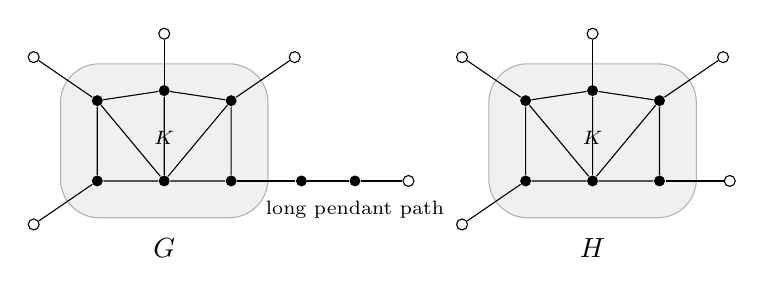
\begin{tikzpicture}[scale=0.85,
  v/.style={circle,fill=black,inner sep=1.4pt},
  l/.style={circle,draw=black,fill=white,inner sep=1.4pt}]
\foreach \dx/\lab/\long in {0/G/1, 6.4/H/0}{
  \begin{scope}[xshift=\dx cm]
  \draw[rounded corners=14pt,fill=gray!12,draw=gray!60] (-1.55,-1.15) rectangle (1.55,1.15);
  \node[v] (a) at (-1,0.6) {}; \node[v] (b) at (0,0.75) {}; \node[v] (c) at (1,0.6) {};
  \node[v] (d) at (-1,-0.6) {}; \node[v] (e) at (0,-0.6) {}; \node[v] (f) at (1,-0.6) {};
  \draw (a)--(b)--(c)--(f)--(e)--(d)--(a) (b)--(e) (a)--(e) (c)--(e);
  \node[l] (la) at (-1.95,1.25) {}; \draw (a)--(la);
  \node[l] (lb) at (0,1.6) {}; \draw (b)--(lb);
  \node[l] (lc) at (1.95,1.25) {}; \draw (c)--(lc);
  \node[l] (ld) at (-1.95,-1.25) {}; \draw (d)--(ld);
  \ifnum\long=1
    \node[v] (p1) at (2.05,-0.6) {}; \node[v] (p2) at (2.85,-0.6) {}; \node[l] (p3) at (3.65,-0.6) {};
    \draw (f)--(p1)--(p2)--(p3);
    \node[below] at (2.85,-0.75) {\scriptsize long pendant path};
  \else
    \node[l] (p1) at (2.05,-0.6) {}; \draw (f)--(p1);
  \fi
  \node at (0,-1.6) {$\lab$};
  \node at (0,0.05) {\scriptsize $K$};
  \end{scope}}
\end{tikzpicture}
\caption{Schematic shape of a minimal counterexample $G$ (left) and of its bag $H$ (right) in
Theorems~\ref{thm:structure} and~\ref{thm:bagred}. Shaded: the bridgeless core $K$; open circles: vertices of degree
one. Every vertex of $K$ carries at most one pendant path, at most one pendant path is long, and $H$ keeps only the first
vertex of each pendant path.}\label{fig:shape}
\end{figure}

\begin{corollary}\label{cor:bagimpliesA}
If~\eqref{B} holds for every bag, then~\eqref{A} holds for every connected graph, and Conjecture~\ref{conj:F} follows.
\end{corollary}

\begin{proof}
Apply Theorems~\ref{thm:structure} and~\ref{thm:bagred} to the class of all connected graphs.
\end{proof}

Cygan, Pilipczuk and \v{S}krekovski observed that the general bag inequality would imply Conjecture~\ref{conj:F}.
Their reduction is different (it treats all bridgeless components of a minimal counterexample simultaneously); the
proof above is self-contained and works inside any admissible class, which is what Section~\ref{sec:bags} needs.

\section{The bag inequality for small cores, and the main theorem}\label{sec:bags}

\begin{theorem}[Computer-assisted]\label{thm:bagcomp}
Every bag $H$ with $|V(C(H))|\le\kmax$ satisfies~\eqref{B}. Equality holds only when $C(H)=K_{2,3}$ and all five core
vertices carry a pendant vertex.
\end{theorem}

\begin{proof}[Method]
A bag is determined by its core $C$ and the set $U\subseteq V(C)$ of core vertices carrying a pendant vertex. A core
vertex of core-degree at most three, or without a core neighbour of smaller core-degree, must lie in $U$: otherwise it is
locally minimal in $H$ (for core-degree two directly; then for core-degree three, since all core vertices have degree at
least three; and in the last case because $d_H(v)=d_C(v)\le d_C(w)\le d_H(w)$ for all neighbours $w$), and its core
edges are not supportive by Lemma~\ref{lem:locmin}. The program \texttt{bags2.c} (Appendix~\ref{app:code}) reads all
connected graphs with minimum degree at least two produced by \texttt{geng -c -d2}~\cite{nauty}, keeps the bridgeless
ones, and for each of them runs through all sets $U$ containing the forced vertices. Condition (3) of
Definition~\ref{def:bag} is tested exactly with Lemma~\ref{lem:edge} in integer arithmetic, and $\Rp(H)$ is computed exactly
as an integer multiple of $1/27720$ ($27720=\mathrm{lcm}(1,\dots,11)$, and all degrees are at most $11$).
Table~\ref{tab:bags} records the outcome. Core order $10$ takes about $42$ seconds on one core; for core order $11$ the
input was split into eight parts with \texttt{geng}'s \texttt{res/mod} option, each taking about 13 to 18 minutes on one
core. An independent brute-force script (Appendix~\ref{app:code}), which uses no forced
vertices and no deletion formula but tries every $U\subseteq V(C)$ and recomputes $\Rp(H-e)$ for every core edge with
rational arithmetic, reproduces the numbers of cores and bags, the minimum slack and the minimum drop for every core order
up to $7$. A variant of \texttt{bags2.c} that forces only the vertices of core-degree at most three (and therefore
enumerates more sets $U$) gives identical results for every core order up to $10$.
\end{proof}

\begin{table}[ht]
\centering
\small
\begin{tabular}{rrrccc}
\toprule
$|V(C)|$ & bridgeless cores & bags & min slack in \eqref{B} & min drop & min $|U|$\\
\midrule
3 & 1 & 0 & -- & -- & --\\
4 & 3 & 1 & $5/12$ & $3/4$ & 4\\
5 & 11 & 5 & $0$ & $1$ & 3\\
6 & 60 & 12 & $1/3$ & $17/20$ & 4\\
7 & 502 & 80 & $2/3$ & $59/60$ & 4\\
8 & 7\,403 & 504 & $2/3$ & $13/15$ & 5\\
9 & 197\,442 & 5\,468 & $1$ & $1$ & 4\\
10 & 9\,804\,368 & 82\,715 & $1$ & $19/21$ & 4\\
11 & 902\,818\,087 & 1\,731\,733 & $4/3$ & $1$ & 4\\
\bottomrule
\end{tabular}
\medskip
\caption{All bags with small cores. ``Slack'' is $\Rp(H)-\rad(C)-1$; it is never negative, and it is zero only for
$K_{2,3}$ with five pendant vertices. ``Drop'' is $\Rp(H)-\Rp(C)$, and $|U|$ is the number of pendant vertices. The numbers of bridgeless cores agree with
the numbers of connected bridgeless graphs (OEIS A007146~\cite{OEIS2}).}\label{tab:bags}
\end{table}

\begin{figure}[ht]
\centering
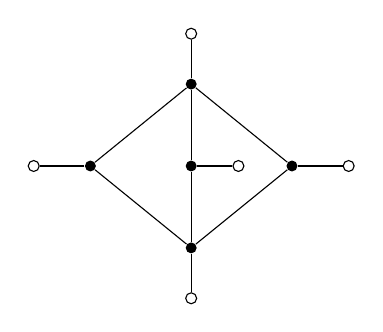
\begin{tikzpicture}[scale=0.8,
  v/.style={circle,fill=black,inner sep=1.4pt},
  l/.style={circle,draw=black,fill=white,inner sep=1.4pt}]
\node[v] (x1) at (0,1.3) {}; \node[v] (x2) at (0,-1.3) {};
\node[v] (y1) at (-1.6,0) {}; \node[v] (y2) at (0,0) {}; \node[v] (y3) at (1.6,0) {};
\foreach \y in {y1,y2,y3}{\draw (x1)--(\y)--(x2);}
\node[l] (px1) at (0,2.1) {}; \draw (x1)--(px1);
\node[l] (px2) at (0,-2.1) {}; \draw (x2)--(px2);
\node[l] (py1) at (-2.5,0) {}; \draw (y1)--(py1);
\node[l] (py2) at (0.75,0) {}; \draw (y2)--(py2);
\node[l] (py3) at (2.5,0) {}; \draw (y3)--(py3);
\end{tikzpicture}
\caption{The only bag with core order at most $\kmax$ attaining equality in~\eqref{B}: $K_{2,3}$ with a pendant vertex at
each of its five vertices; $\Rp(H)=3=\rad(K_{2,3})+1$.}\label{fig:k23}
\end{figure}

For the equality case, $H$ consists of $K_{2,3}$ (parts $\{x_1,x_2\}$ and $\{y_1,y_2,y_3\}$) with a pendant vertex at
each of the five vertices; then $d_{x_i}=4$, $d_{y_j}=3$, $\Rp(H)=6\cdot\frac14+2\cdot\frac14+3\cdot\frac13=3=\rad(K_{2,3})+1$,
and every core edge $y_jx_i$ has $a_{y_j}-b_{x_i}=\frac16-0>0$.

\begin{lemma}\label{lem:admissible}
For integers $k\ge1$ and $m\ge0$ let $\C(k,m)$ be the class of connected graphs $G$ such that every two-edge-connected
component $B$ of $G$ with at least two vertices satisfies $|V(B)|\le k$, or $\mu(B)\le m$, or $d_G(v)\le4$ for all
$v\in V(B)$. Then $\C(k,m)$ is admissible.
\end{lemma}

\begin{proof}
Let $G'$ be a connected subgraph of $G\in\C(k,m)$. A two-edge-connected component $B'$ of $G'$ with at least two vertices
is a two-edge-connected subgraph of $G$, so it is contained in a two-edge-connected component $B$ of $G$. Then
$|V(B')|\le|V(B)|$; $\mu(B')\le\mu(B)$, because $B$ arises from its connected subgraph $B'$ by adding vertices, each
with at least one new edge, and further edges; and $d_{G'}(v)\le d_G(v)$. So $B'$ satisfies the same alternative as $B$.
The graph $G'$ of Lemma~\ref{lem:replace} consists of the connected subgraph $G_x$ of $G$ and a pendant path at $x$; its
two-edge-connected components with at least two vertices are those of $G_x$, and all degrees of vertices of $G_x$ in $G'$
are at most their degrees in $G$.
\end{proof}

\begin{theorem}[Main theorem]\label{thm:main}
Every graph $G\in\C(\kmax,\mumax)$ satisfies~\eqref{A}. That is, if every two-edge-connected component $B$ of a connected
graph $G$ has at most $\kmax$ vertices, or cyclomatic number at most $\mumax$, or only vertices of degree at most four in
$G$, then $\Rp(G)\ge\rad(G)-\frac12$, hence $R(G)\ge\rad(G)-\frac12$ and Conjecture~\ref{conj:F} holds for $G$.
\end{theorem}

\begin{proof}
Suppose not, and let $G\in\C(\kmax,\mumax)$ be a counterexample with $|V(G)|$ and then $|E(G)|$ minimal. By
Lemma~\ref{lem:admissible} and Theorem~\ref{thm:structure}, the core $K$ is a two-edge-connected component of $G$.
If $\mu(K)\le\mumax$, then $|V(K)|\le2\mu(K)+1\le\kmax$ by Theorem~\ref{thm:structure}(f). So either
$|V(K)|\le\kmax$, and Theorem~\ref{thm:bagcomp} gives~\eqref{B} for the bag $H$ of Theorem~\ref{thm:bagred}; or all
vertices of $K$ have degree at most four in $G$, hence in $H$, so $H$ has maximum degree at most four and~\eqref{B}
holds by~\cite[Proposition~4.3]{CPS}. Both contradict Theorem~\ref{thm:bagred}.
\end{proof}

\begin{remark}
Theorem~\ref{thm:main} uses Theorem~\ref{thm:bagcomp} only for cores that can occur in Theorem~\ref{thm:bagred}. Using the
additional restrictions of Theorem~\ref{thm:structure}, for example $\Rp(H)-\Rp(K)<1$ when there is no long pendant path,
would shrink the search considerably; we did not need this for core order at most $\kmax$.
\end{remark}

\section{A conservation identity for supportive edges}\label{sec:conservation}

In this section $G$ is a graph and $Q\subseteq V(G)$ is a nonempty set of vertices of degree at least two such that
\begin{equation}\label{EXT}\tag{EXT}
\text{every neighbour outside $Q$ of a vertex $v\in Q$ has degree smaller than $d_v$.}
\end{equation}
For $v\in Q$ let $p_v=|N(v)\setminus Q|$ (the number of \emph{external} neighbours), let $L_Q(v)$ and $U_Q(v)$ be the
sets of neighbours of $v$ in $Q$ of smaller and of larger degree, and let $e_v$ be the number of neighbours of $v$ in $Q$
of degree $d_v$. By~\eqref{EXT}, $\lambda_v=p_v+|L_Q(v)|$ and $h_v=e_v+|U_Q(v)|$. An edge $uv$ of $G[Q]$ with $d_u<d_v$
is \emph{strict}. For $D\subseteq Q$ the \emph{injection} into $D$ is $I(D)=\sum_{v\in D}p_vb_v$.

\begin{theorem}[Conservation identity]\label{thm:conservation}
\[
I(Q)=\sum_{\substack{uv\in E(G[Q])\\ d_u<d_v}}\bigl(a_u-b_v\bigr)\;+\;\sum_{v\in Q}e_v\,a_v .
\]
\end{theorem}

\begin{proof}
For every $v$, $\lambda_vb_v=\lambda_vh_v/g_v=h_va_v$. Summing over $Q$,
\[
\sum_{v\in Q}\bigl(p_v+|L_Q(v)|\bigr)b_v=\sum_{v\in Q}\bigl(e_v+|U_Q(v)|\bigr)a_v .
\]
Now $\sum_v|L_Q(v)|b_v$ is the sum of $b_v$ over all strict edges $uv$ ($d_u<d_v$), and $\sum_v|U_Q(v)|a_v$ is the sum
of $a_u$ over the same edges.
\end{proof}

By Lemma~\ref{lem:edge}(i), $a_u-b_v=\Rp(G-uv)-\Rp(G)$ for a strict edge, so if all strict edges of $G[Q]$ are
supportive, the injection $I(Q)$ is a sum of positive ``slacks'' of strict edges and nonnegative contributions of
equal-degree edges. For a bag $H$ with core $C$ and pendant set $U$, take $Q=V(C)$; then $p_v=1$ for $v\in U$ and
$p_v=0$ otherwise, and Lemma~\ref{lem:leaves} gives
\begin{equation}\label{eq:drop}
\Rp(H)-\Rp(C)=I(V(C))-\sum_{\substack{uv\in E(C),\ u,v\in U\\ d_u=d_v}}\frac1{g_u} .
\end{equation}

We read Theorem~\ref{thm:conservation} as a flow statement. Give each strict edge $uv$ ($d_u<d_v$) the flow $a_u$ from
$u$ to $v$, and put $\mathrm{In}(v)=\sum_{u\in L_Q(v)}a_u$ and $\mathrm{Out}(v)=|U_Q(v)|\,a_v$.

\begin{lemma}[Local conservation]\label{lem:flow}
If every strict edge of $G[Q]$ is supportive, then for every $v\in Q$
\[
\mathrm{Out}(v)+e_va_v\ \le\ \mathrm{In}(v)+p_vb_v ,
\]
with strict inequality whenever $L_Q(v)\ne\emptyset$.
\end{lemma}

\begin{proof}
$\mathrm{Out}(v)+e_va_v=h_va_v=\lambda_vb_v=p_vb_v+|L_Q(v)|\,b_v$, and $b_v<a_u$ for every $u\in L_Q(v)$ by
Lemma~\ref{lem:edge}(i).
\end{proof}

Call $D\subseteq Q$ a \emph{down-set} if $L_Q(v)\subseteq D$ for every $v\in D$.

\begin{lemma}[Cut inequality]\label{lem:cut}
If every strict edge of $G[Q]$ is supportive and $D$ is a down-set, then
\[
\sum_{\substack{u\in D,\ v\in U_Q(u)\setminus D}}a_u\;+\;\sum_{v\in D}e_va_v\ \le\ I(D).
\]
\end{lemma}

\begin{proof}
Sum Lemma~\ref{lem:flow} over $D$. Because $D$ is a down-set, $\sum_{v\in D}\mathrm{In}(v)$ is the total flow on
strict edges inside $D$, which is also part of $\sum_{v\in D}\mathrm{Out}(v)$; the rest of that sum is the flow leaving $D$.
\end{proof}

Let $\preceq$ be the reflexive--transitive closure of the relation ``$u\in L_Q(v)$''. Degrees increase strictly along
$\prec$, so $\preceq$ is a partial order on $Q$. For $A\subseteq Q$ let $\downarrow\!A=\{v\in Q: v\preceq a\text{ for some }a\in A\}$.

\begin{theorem}[Antichain inequality]\label{thm:antichain}
If every strict edge of $G[Q]$ is supportive, then every antichain $A$ of $(Q,\preceq)$ satisfies
\[
\sum_{a\in A}\lambda_a b_a\ \le\ I(\downarrow\!A),\qquad\text{and in particular}\qquad
\sum_{\substack{a\in A\\ \lambda_a\ge1,\ h_a\ge1}}\frac1{d_a}\ \le\ I(\downarrow\!A).
\]
\end{theorem}

\begin{proof}
Let $D=\downarrow\!A\setminus A$. If $v\in D$ and $u\in L_Q(v)$, then $u\prec v\preceq a$ for some $a\in A$, so
$u\in\downarrow\!A$, and $u\notin A$ since $A$ is an antichain; thus $D$ is a down-set. For $a\in A$ we have
$L_Q(a)\subseteq D$ by the same argument, so the edges into $A$ from below leave $D$, and Lemma~\ref{lem:cut} gives
$\sum_{a\in A}\mathrm{In}(a)\le I(D)$. By Lemma~\ref{lem:edge}(i),
$\lambda_ab_a=p_ab_a+|L_Q(a)|b_a\le p_ab_a+\mathrm{In}(a)$. Summing over $A$ proves the first inequality. For the second,
$\lambda_ah_a\ge\lambda_a+h_a-1=d_a-1$ when $\lambda_a,h_a\ge1$, so $\lambda_ab_a\ge 1/d_a$.
\end{proof}

\begin{corollary}[A single supported vertex]\label{cor:single}
Suppose $G[Q]$ is connected, every edge of $G[Q]$ is supportive, one vertex $q\in Q$ has $p_q=1$, all other vertices of
$Q$ have $p_v=0$, and every vertex of $Q\setminus\{q\}$ has a neighbour of smaller degree in $Q$. Then $q\prec v$, and
hence $d_q<d_v$, for all $v\in Q\setminus\{q\}$; every vertex of $Q\setminus\{q\}$ has degree larger than $d_q(d_q-1)$; and every antichain
$A\subseteq Q\setminus\{q\}$ satisfies $\sum_{a\in A,\,h_a\ge1}1/d_a\le 1/d_q$.
\end{corollary}

\begin{proof}
Following lower neighbours from any $v\neq q$ ends at a vertex without lower neighbour in $Q$, which must be $q$; so
$q\prec v$. Hence all neighbours of $q$ in $Q$ are higher, $\lambda_q=1$, $h_q=d_q-1$ and $I(Q)=b_q=1/d_q$. A vertex
$w\ne q$ of minimum degree in $Q\setminus\{q\}$ can only have $q$ as a lower neighbour, so $\lambda_w=1$, $b_w=1/d_w$,
and supportiveness of $qw$ means $\frac1{d_q(d_q-1)}=a_q>b_w=\frac1{d_w}$. The last claim is
Theorem~\ref{thm:antichain}.
\end{proof}

Let us call a \emph{configuration} a connected graph $Q$ together with $U\subseteq V(Q)$; put $p_v=1$ for $v\in U$ and
$p_v=0$ otherwise, $d_v=d_Q(v)+p_v$, and call it \emph{valid} if $d_v\ge2$ for all $v$, every vertex outside $U$ has a
neighbour of smaller degree in $Q$, and every edge of $Q$ is supportive when each external neighbour is regarded as a
lower neighbour. By Theorem~\ref{thm:structure}, the core $K$ of a minimal counterexample to~\eqref{A}, with $U$ the set
of vertices carrying a pendant path, is a valid configuration.

\begin{proposition}[Computer-assisted]\label{prop:fewsupport}
For $3\le|V(Q)|\le11$ there is no valid configuration with $|U|\le2$. For $|V(Q)|=2$ the only valid configuration with
$|U|\le2$ is $Q=K_2$ with $U=V(Q)$, i.e.\ the path $P_4$.
\end{proposition}

\begin{proof}[Method]
The program \texttt{lemu.c} (Appendix~\ref{app:code}) tests every connected graph $Q$ on $n\le11$ vertices produced by
\texttt{geng -c} and every $U$ with $|U|\in\{1,2\}$, using the exact test of Lemma~\ref{lem:edge}.
\end{proof}

Hence a minimal counterexample to~\eqref{A} whose core has at most $11$ vertices has at least three pendant paths, and,
by Table~\ref{tab:bags}, every bag with at most $\kmax$ core vertices has at least three pendant vertices.

\section{Exhaustive verification through eleven vertices}\label{sec:exhaustive}

\begin{theorem}[Computer-assisted]\label{thm:exhaustive}
Let $G$ be a connected graph with $2\le|V(G)|\le11$. Then:
\begin{enumerate}[(a)]
\item $\Rp(G)\ge\rad(G)-\frac12$; whenever equality holds, $\diam(G)=2\rad(G)-1$;
\item if $G$ has at most one vertex of degree one, then $\Rp(G)\ge\rad(G)$;
\item if $G$ is not a path on an even number $n\ge4$ of vertices, then $R(G)\ge\rad(G)$, with equality if and only if
$G\in\{K_2,C_4,C_6,C_8,C_{10}\}$; otherwise $R(G)-\rad(G)\ge0.2700556$.
\end{enumerate}
\end{theorem}

\begin{proof}[Method]
The program \texttt{verify.c} (Appendix~\ref{app:code}) reads the output of \texttt{geng -c $n$} for $n\le11$. The radius is
computed by bit-parallel breadth-first search. For $n\le11$ every degree is at most $10$, so $2520\,\Rp(G)$ is an integer
($2520=\mathrm{lcm}(1,\dots,10)$), and (a) and (b) are decided in exact integer arithmetic. For (c), $R(G)$ is a sum of at
most $55$ terms $1/\sqrt{d_ud_v}$, each computed with correctly rounded square root and division, so the computed sum has
absolute error below $10^{-12}$; all graphs with $|R(G)-\rad(G)|<10^{-9}$ are printed and turn out to be exactly
$K_2,C_4,C_6,C_8,C_{10}$, for which $R=\rad$ holds exactly. The diameter statement in (a) was checked on the list of all
equality graphs. The case $n=11$ was split into two halves with \texttt{geng}'s \texttt{res/mod} option; each half took about six and a
half minutes on one core. The counts of graphs
agree with the numbers of connected graphs (OEIS A001349~\cite{OEIS}). Table~\ref{tab:exh} summarizes the run. An
independent Python script (Appendix~\ref{app:code}) with exact rational arithmetic and \texttt{networkx} reproduces all
counts of Table~\ref{tab:exh} and the equality graphs in (c) for $n\le8$.
\end{proof}

\begin{table}[ht]
\centering
\small
\begin{tabular}{rrrrrc}
\toprule
$n$ & connected graphs & eq.\ in \eqref{A} & $\le1$ leaf & eq.\ in $\Rp\ge\rad$ & min $R-\rad$\\
\midrule
2 & 1 & 0 & 0 & 0 & -- \\
3 & 2 & 0 & 1 & 0 & $0.4142136$\\
4 & 6 & 1 & 4 & 1 & $0.7320508$\\
5 & 21 & 1 & 16 & 4 & $0.2700556$\\
6 & 112 & 2 & 90 & 3 & $0.5606602$\\
7 & 853 & 4 & 731 & 7 & $0.2700556$\\
8 & 11\,117 & 9 & 10\,108 & 11 & $0.5606602$\\
9 & 261\,080 & 17 & 248\,551 & 19 & $0.2700556$\\
10 & 11\,716\,571 & 38 & 11\,461\,640 & 33 & $0.5606602$\\
11 & 1\,006\,700\,565 & 75 & 997\,820\,259 & 52 & $0.2700556$\\
\bottomrule
\end{tabular}
\medskip
\caption{Exhaustive verification. Columns: number of connected graphs; number with equality in~\eqref{A}; number with at
most one vertex of degree one; number of those with $\Rp=\rad$; minimum of $R(G)-\rad(G)$ over graphs other than even
paths and the equality graphs $K_2,C_4,\dots,C_{10}$. No violation of~\eqref{A}, of $\Rp\ge\rad$ for graphs with at most
one leaf, or of Conjecture~\ref{conj:CH} occurs. For odd $n\ge5$ it is attained by a path with two leaves attached at one
end, where $R-\rad=\frac2{\sqrt3}+\frac1{\sqrt6}+\frac1{\sqrt2}-2$.}\label{tab:exh}
\end{table}

The equality graphs of~\eqref{A} include the even paths, the stars with one subdivided edge, and for $n\ge7$ also
graphs with cycles; all of them are extremal for Theorem~\ref{thm:DLS} with odd diameter. The graphs with at most one leaf
and $\Rp(G)=\rad(G)$ include the even cycles and the complete bipartite graphs $K_{2,m}$.

\section{Conjectures and the remaining gap}\label{sec:open}

The first conjecture is the general form of~\cite[Proposition 4.3]{CPS}. By Corollary~\ref{cor:bagimpliesA} it
implies~\eqref{A} and therefore Conjecture~\ref{conj:F}.

\begin{conjecture}[Bag inequality]\label{conj:bag}
Every bag $H$ satisfies $\Rp(H)\ge\rad(C(H))+1$.
\end{conjecture}

Evidence: Theorem~\ref{thm:bagcomp} and the proof of~\cite{CPS} for maximum degree four. The difficulty is visible in
Table~\ref{tab:bags}. One would like to combine a bound $\Rp(C)\ge\rad(C)$ for the bridgeless core (which holds for all
bridgeless graphs on at most $11$ vertices by Theorem~\ref{thm:exhaustive}(b)) with a bound $\Rp(H)-\Rp(C)\ge1$ for the
drop~\eqref{eq:drop}. The drop, however, can be as small as $\frac34$, and the slack in~\eqref{B} vanishes for
$K_{2,3}$; so the two parts cannot be separated, and the core and the pendant set must be treated together.
Theorem~\ref{thm:conservation} expresses the drop through the slacks of the strict core edges, which is the form in which
the supportive condition enters.
Table~\ref{tab:byrad} suggests that the slack in~\eqref{B} grows with the order of the core: for each value of the radius,
the minimum of $\Rp(H)$ increases with $|V(C)|$, roughly by $\frac13$ per vertex. For radius two and core order
$5\le|V(C)|\le8$ the minimum is attained by $K_{2,m}$ with a pendant vertex at each of its $m$ vertices of degree two
(for $m=3$ also at the other two vertices; for $m\ge4$ pendant vertices there do not change the value), where
$\Rp(H)=2+\frac m3$.

\begin{table}[ht]
\centering
\small
\begin{tabular}{rcccc}
\toprule
$|V(C)|$ & $\rad(C)=1$ & $\rad(C)=2$ & $\rad(C)=3$ & $\rad(C)=4$\\
\midrule
4 & $29/12$ & -- & -- & --\\
5 & $11/4$ & $3$ & -- & --\\
6 & $47/15$ & $10/3$ & -- & --\\
7 & $7/2$ & $11/3$ & -- & --\\
8 & $107/28$ & $4$ & $14/3$ & --\\
9 & $33/8$ & $361/84$ & $5$ & --\\
10 & $53/12$ & $55/12$ & $16/3$ & $6$\\
\bottomrule
\end{tabular}
\medskip
\caption{Minimum of $\Rp(H)$ over all bags $H$ with given core order and core radius (exact values). The bag
inequality~\eqref{B} asks for at least $\rad(C)+1$, that is $2,3,4,5$ in the four columns. Computed by a variant of
\texttt{bags2.c} that records the minimum of $\Rp(H)$ separately for each value of $\rad(C)$.}\label{tab:byrad}
\end{table}

\begin{conjecture}[One leaf]\label{conj:oneleaf}
Every connected graph with at most one vertex of degree one satisfies $\Rp(G)\ge\rad(G)$.
\end{conjecture}

Since $R\ge\Rp$, Conjecture~\ref{conj:oneleaf} would give Conjecture~\ref{conj:CH} for all graphs with at most one leaf,
in particular for all graphs of minimum degree at least two. It holds for $n\le11$ (Theorem~\ref{thm:exhaustive}(b)),
with equality for the even cycles and the graphs $K_{2,m}$ among others. A randomized local search (simulated annealing
over edge toggles, program \texttt{sa\_oneleaf.c} in Appendix~\ref{app:code}) on graphs with $13$ to $30$ vertices found
no violation of Conjecture~\ref{conj:oneleaf} or of~\eqref{A}; this is weak evidence, since such searches tend to stay
near the many equality graphs.

\begin{remark}[Few supports]\label{conj:few}
Is there a valid configuration with $|V(Q)|\ge3$ and $|U|\le2$? None exists with $|V(Q)|\le11$
(Proposition~\ref{prop:fewsupport}), but for the case relevant to bags this is no evidence at all. Consider a valid
configuration with $U=\{q\}$ and $d_q\ge3$ (in a bag or in the core of a minimal counterexample, $d_q\ge3$). By
Corollary~\ref{cor:single} every other vertex has degree at least $m>d_q(d_q-1)$. Let $L_1$ be the set of vertices whose only
lower neighbour is $q$; then $L_1\subseteq N(q)$, so $|L_1|\le d_q-1$, and $Q\neq\{q\}\cup L_1$ because degrees exceed
$|L_1|$. A vertex $w$ of minimum degree $k$ in $Q\setminus(\{q\}\cup L_1)$ has all its lower neighbours in $\{q\}\cup L_1$, at
least one of them, $u$, in $L_1$; hence $\lambda_w\le d_q$ and supportiveness of $uw$ gives
$\frac{k-d_q}{k(k-1)}\le b_w<a_u=\frac1{d_u(d_u-1)}\le\frac1{m(m-1)}$. For $d_q\ge3$ (so $m\ge7$) this forces $k\ge40$, hence
$|V(Q)|\ge41$. A negative answer to the question would imply that every bag has at least three pendant vertices and that a
minimal counterexample to~\eqref{A} has at least three pendant paths.
\end{remark}

\subsection*{Summary of the gap}
A proof of~\eqref{A}, and hence of Conjecture~\ref{conj:F}, along the present lines requires Conjecture~\ref{conj:bag}
for cores of every order, whereas we can certify it only for cores of order at most $\kmax$. The minimal counterexample
analysis (Theorem~\ref{thm:structure}) and the conservation identity (Theorem~\ref{thm:conservation}) reduce the problem
to this single family of inequalities but do not prove them.

\appendix
\section{Programs}\label{app:code}

All computations used \texttt{geng} from nauty~2.8.8~\cite{nauty}, compiled C (\texttt{gcc -O3}), and Python~3 with
\texttt{networkx} for the cross-checks. The listings below are complete. Typical invocations:
\begin{lstlisting}[frame=none]
geng -cq 11 0/2 | ./verify          # half of the 11-vertex connected graphs
geng -cq -d2 10 | ./bags2           # all bags with 10-vertex cores
geng -cq -d2 11 3/8 | ./bags2       # one eighth of the 11-vertex cores
geng -cq 11 | ./lemu                # configurations with |U| <= 2
\end{lstlisting}

\medskip\noindent\textbf{A.1.} \texttt{verify.c} (Theorem~\ref{thm:exhaustive})\par\nobreak
\begin{lstlisting}[language=C]
/* verify.c -- exhaustive check of radius inequalities for the Randic index R and the
 * modified Randic index R'(G) = sum_{uv in E} 1/max(d(u),d(v)).
 *
 *   (A)  R'(G) >= rad(G) - 1/2                for every connected graph G     [implies Fajtlowicz]
 *   (A1) R'(G) >= rad(G)  if G has at most one vertex of degree 1
 *   (CH) R(G)  >= rad(G)  unless G is a path on an even number >= 4 of vertices [Caporossi-Hansen]
 *
 * Input: graph6 strings, one per line (e.g. nauty: geng -cq n | ./verify).
 * (A),(A1): exact integer arithmetic.  For n <= 11 every degree is <= 10 and 2520 = lcm(1..10),
 *           so 2520*R'(G) is an integer.  Graphs with a vertex of degree > 10 are rejected.
 * (CH):     R is summed in IEEE double precision.  Every term 1/sqrt(d_u d_v) is computed with
 *           correctly rounded sqrt and division, and at most 55 terms are added, so the absolute
 *           error of the computed sum is far below 1e-12.  Graphs with |R - rad| < 1e-9 are
 *           printed (tag NEAR) and decided separately in exact arithmetic.
 */
#include <stdio.h>
#include <stdlib.h>
#include <string.h>
#include <math.h>

#define MAXN 16
#define SCALE 2520

static int n, deg[MAXN];
static unsigned nb[MAXN];
static double isq[MAXN][MAXN];

static void parse(const char *s) {
    int p = 0;
    n = s[p++] - 63;
    if (n < 1 || n > MAXN) { fprintf(stderr, "bad order\n"); exit(1); }
    memset(deg, 0, sizeof deg); memset(nb, 0, sizeof nb);
    int bits = 0, val = 0;
    for (int j = 1; j < n; j++)
        for (int i = 0; i < j; i++) {
            if (bits == 0) { val = s[p++] - 63; bits = 6; }
            bits--;
            if ((val >> bits) & 1) { nb[i] |= 1u << j; nb[j] |= 1u << i; deg[i]++; deg[j]++; }
        }
}

/* radius by bit-parallel BFS; returns -1 if the graph is disconnected */
static int radius(void) {
    unsigned all = (n == 32) ? 0xffffffffu : ((1u << n) - 1);
    int best = 1 << 30;
    for (int s = 0; s < n; s++) {
        unsigned seen = 1u << s, fr = 1u << s; int e = 0;
        while (seen != all) {
            unsigned nx = 0;
            for (unsigned f = fr; f; f &= f - 1) nx |= nb[__builtin_ctz(f)];
            nx &= ~seen;
            if (!nx) return -1;
            seen |= nx; fr = nx; e++;
            if (e >= best) break;          /* cannot improve the minimum */
        }
        if (e < best) best = e;
    }
    return best;
}

int main(void) {
    char line[256];
    for (int a = 1; a < MAXN; a++) for (int b = 1; b < MAXN; b++) isq[a][b] = 1.0 / sqrt((double)(a * b));
    long long cnt = 0, eqA = 0, violA = 0, cntA1 = 0, eqA1 = 0, violA1 = 0, violCH = 0, nearCH = 0, evenpaths = 0;
    long long minA = 1LL << 60, minA1 = 1LL << 60;
    double minCH = 1e9;
    char wCH[256] = "";
    while (fgets(line, sizeof line, stdin)) {
        int len = (int)strlen(line);
        while (len && (line[len - 1] == '\n' || line[len - 1] == '\r')) line[--len] = 0;
        parse(line);
        if (n < 2) continue;
        int r = radius();
        if (r < 0) { fprintf(stderr, "disconnected input %s\n", line); return 1; }
        long long S = 0; int leaves = 0, deg2 = 0, m = 0; double R = 0.0;
        for (int i = 0; i < n; i++) {
            if (deg[i] > 10) { fprintf(stderr, "degree > 10 not supported\n"); return 1; }
            if (deg[i] == 1) leaves++;
            if (deg[i] == 2) deg2++;
            for (unsigned f = nb[i] & ~((2u << i) - 1); f; f &= f - 1) {   /* neighbours j > i */
                int j = __builtin_ctz(f);
                int mx = deg[i] > deg[j] ? deg[i] : deg[j];
                S += SCALE / mx; R += isq[deg[i]][deg[j]]; m++;
            }
        }
        cnt++;
        /* (A) */
        long long sA = S - (long long)SCALE * r + SCALE / 2;
        if (sA < minA) minA = sA;
        if (sA < 0) { violA++; printf("VIOLATION(A) %s\n", line); } else if (sA == 0) eqA++;
        /* (A1) */
        if (leaves <= 1) {
            cntA1++;
            long long s1 = S - (long long)SCALE * r;
            if (s1 < minA1) minA1 = s1;
            if (s1 < 0) { violA1++; printf("VIOLATION(A1) %s\n", line); } else if (s1 == 0) eqA1++;
        }
        /* (CH) */
        int evenpath = (n >= 4 && n % 2 == 0 && m == n - 1 && leaves == 2 && deg2 == n - 2);
        if (evenpath) { evenpaths++; continue; }
        double sc = R - r;
        if (sc < minCH) { minCH = sc; strcpy(wCH, line); }
        if (fabs(sc) < 1e-9) { nearCH++; printf("NEAR(CH) %s r=%d R=%.15f\n", line, r, R); }
        else if (sc < 0) { violCH++; printf("VIOLATION(CH) %s r=%d R=%.15f\n", line, r, R); }
    }
    printf("SUMMARY graphs %lld | (A) min 2520*(R'-rad+1/2) = %lld, equality %lld, violations %lld"
           " | (A1) graphs with <=1 leaf %lld, min 2520*(R'-rad) = %lld, equality %lld, violations %lld"
           " | (CH) even paths skipped %lld, min R-rad = %.9f at %s, near-equality %lld, violations %lld\n",
           cnt, minA, eqA, violA, cntA1, cntA1 ? minA1 : 0, eqA1, violA1, evenpaths, minCH, wCH, nearCH, violCH);
    return 0;
}
\end{lstlisting}

\medskip\noindent\textbf{A.2.} \texttt{bags2.c} (Theorem~\ref{thm:bagcomp})\par\nobreak
\begin{lstlisting}[language=C]
/* bags2.c -- exhaustive check of the bag inequality R'(H) >= rad(C(H)) + 1 for every bag H whose core C(H)
 * has a given number n <= 11 of vertices.  Input: graph6 strings of all connected graphs with minimum degree
 * >= 2 (geng -c -d2 n); graphs with a bridge are skipped.  A bag is a core C plus a set U of core vertices,
 * each carrying one pendant vertex, such that every core edge is supportive (deleting it increases R').
 *
 * Forced pendants.  If a core vertex v has no core neighbour of smaller core-degree, then v must carry a
 * pendant in every bag: otherwise d_H(v) = cdeg(v) <= cdeg(w) <= d_H(w) for every neighbour w, so v is
 * locally minimal in H and its core edges are not supportive.  The same holds when cdeg(v) <= 3 (a vertex
 * of core-degree 2 without pendant is locally minimal; then a vertex of core-degree 3 without pendant has
 * only neighbours of H-degree >= 3).  Inside the enumeration we additionally require (before the exact
 * supportive test) that every core vertex outside U has a neighbour of smaller H-degree; this is implied
 * by the supportive test and only speeds it up.
 * Exact arithmetic: R'(H) is an integer multiple of 1/27720 (27720 = lcm(1,...,11)) for cores of order <= 11.
 */
#include <stdio.h>
#include <stdlib.h>
#include <string.h>
#define MAXN 16
#define SCALE 27720
static int n, cdeg[MAXN], d[MAXN], pend[MAXN];
static unsigned nb[MAXN];
static void parse(const char *s) {
    int p = 0; n = s[p++] - 63;
    if (n < 1 || n > 11) { fprintf(stderr, "order must be <= 11\n"); exit(1); }
    memset(cdeg, 0, sizeof cdeg); memset(nb, 0, sizeof nb);
    int bits = 0, val = 0;
    for (int j = 1; j < n; j++) for (int i = 0; i < j; i++) {
        if (bits == 0) { val = s[p++] - 63; bits = 6; }
        bits--;
        if ((val >> bits) & 1) { nb[i] |= 1u << j; nb[j] |= 1u << i; cdeg[i]++; cdeg[j]++; }
    }
}
static int connected_without(int a, int b) {
    unsigned all = (1u << n) - 1, seen = 1u, fr = 1u;
    while (fr) {
        unsigned nx = 0;
        for (unsigned f = fr; f; f &= f - 1) {
            int u = __builtin_ctz(f); unsigned m = nb[u];
            if (u == a) m &= ~(1u << b);
            if (u == b) m &= ~(1u << a);
            nx |= m;
        }
        nx &= ~seen; seen |= nx; fr = nx;
    }
    return seen == all;
}
static int radius(void) {
    unsigned all = (1u << n) - 1; int best = 1 << 30;
    for (int s = 0; s < n; s++) {
        unsigned seen = 1u << s, fr = 1u << s; int e = 0;
        while (seen != all) {
            unsigned nx = 0;
            for (unsigned f = fr; f; f &= f - 1) nx |= nb[__builtin_ctz(f)];
            nx &= ~seen; seen |= nx; fr = nx; e++;
        }
        if (e < best) best = e;
    }
    return best;
}
static int supportive(int i, int j) {
    int di = d[i], dj = d[j], bi = pend[i], bj = pend[j];
    for (unsigned f = nb[i]; f; f &= f - 1) { int w = __builtin_ctz(f); if (w != j && d[w] < di) bi++; }
    for (unsigned f = nb[j]; f; f &= f - 1) { int w = __builtin_ctz(f); if (w != i && d[w] < dj) bj++; }
    long long mx = di > dj ? di : dj;
    long long A = (long long)bi * dj * (dj - 1) * mx + (long long)bj * di * (di - 1) * mx;
    long long B = (long long)di * (di - 1) * dj * (dj - 1);
    return A > B;
}
int main(void) {
    char line[256];
    long long cores = 0, bags = 0, eq = 0, viol = 0, minpend = 1 << 30;
    long long minslack = 1LL << 60, mindrop = 1LL << 60;
    char wslack[256] = "", wdrop[256] = ""; unsigned wsU = 0, wdU = 0;
    while (fgets(line, sizeof line, stdin)) {
        int len = (int)strlen(line);
        while (len && (line[len - 1] == '\n' || line[len - 1] == '\r')) line[--len] = 0;
        parse(line);
        unsigned forced = 0; int opt[MAXN], no = 0;
        for (int i = 0; i < n; i++) {
            int lowcore = 0;
            for (unsigned f = nb[i]; f; f &= f - 1) if (cdeg[__builtin_ctz(f)] < cdeg[i]) { lowcore = 1; break; }
            if (cdeg[i] <= 3 || !lowcore) forced |= 1u << i; else opt[no++] = i;
        }
        int ok = 1;
        for (int i = 0; i < n && ok; i++)
            for (unsigned f = nb[i] & ~((2u << i) - 1); f && ok; f &= f - 1)
                if (!connected_without(i, __builtin_ctz(f))) ok = 0;
        if (!ok) continue;
        cores++;
        int rc = -1; long long Mcore = 0;
        for (unsigned mask = 0; mask < (1u << no); mask++) {
            unsigned U = forced;
            for (int k = 0; k < no; k++) if ((mask >> k) & 1) U |= 1u << opt[k];
            for (int i = 0; i < n; i++) { pend[i] = (U >> i) & 1; d[i] = cdeg[i] + pend[i]; }
            int good = 1;
            for (int i = 0; i < n && good; i++) {           /* quick necessary condition */
                if (pend[i]) continue;
                int has = 0;
                for (unsigned f = nb[i]; f; f &= f - 1) if (d[__builtin_ctz(f)] < d[i]) { has = 1; break; }
                if (!has) good = 0;
            }
            for (int i = 0; i < n && good; i++)
                for (unsigned f = nb[i] & ~((2u << i) - 1); f && good; f &= f - 1)
                    if (!supportive(i, __builtin_ctz(f))) good = 0;
            if (!good) continue;
            if (rc < 0) {
                rc = radius();
                for (int i = 0; i < n; i++)
                    for (unsigned f = nb[i] & ~((2u << i) - 1); f; f &= f - 1) {
                        int j = __builtin_ctz(f); int mx = cdeg[i] > cdeg[j] ? cdeg[i] : cdeg[j]; Mcore += SCALE / mx;
                    }
            }
            bags++;
            if (__builtin_popcount(U) < minpend) minpend = __builtin_popcount(U);
            long long M = 0;
            for (int i = 0; i < n; i++) {
                if (pend[i]) M += SCALE / d[i];
                for (unsigned f = nb[i] & ~((2u << i) - 1); f; f &= f - 1) {
                    int j = __builtin_ctz(f); int mx = d[i] > d[j] ? d[i] : d[j]; M += SCALE / mx;
                }
            }
            long long slack = M - (long long)SCALE * (rc + 1);
            if (slack < minslack) { minslack = slack; strcpy(wslack, line); wsU = U; }
            if (slack < 0) { viol++; printf("VIOLATION %s U=%x\n", line, U); }
            else if (slack == 0) { eq++; printf("EQUALITY %s U=%x\n", line, U); }
            long long drop = M - Mcore;
            if (drop < mindrop) { mindrop = drop; strcpy(wdrop, line); wdU = U; }
        }
    }
    printf("SUMMARY cores %lld bags %lld | min %d*(R'(H)-rad(C)-1) = %lld at %s U=%x | equality %lld violations %lld"
           " | min %d*(R'(H)-R'(C)) = %lld at %s U=%x | min #pendants %lld\n",
           cores, bags, SCALE, bags ? minslack : 0, wslack, wsU, eq, viol, SCALE, bags ? mindrop : 0, wdrop, wdU,
           bags ? minpend : 0);
    return 0;
}
\end{lstlisting}

\medskip\noindent\textbf{A.3.} \texttt{bags\_xcheck.py} (independent cross-check of Theorem~\ref{thm:bagcomp} for core order $\le7$)\par\nobreak
\begin{lstlisting}[language=Python]
"""Independent brute-force cross-check of bags.c for small cores (no shortcuts, no edge-deletion formula).
For every bridgeless connected graph C on n vertices and EVERY subset U of V(C), build H = C + one pendant
vertex at each u in U, test the bag conditions directly (recomputing R' after each core-edge deletion),
and record R'(H) - rad(C) - 1 and R'(H) - R'(C) as exact fractions."""
import sys, itertools, subprocess
from fractions import Fraction as F
import networkx as nx

def Rp(G):
    return sum(F(1, max(G.degree(u), G.degree(v))) for u, v in G.edges())

def main(n, geng):
    out = subprocess.run([geng, '-cq', '-d2', str(n)], capture_output=True, text=True).stdout.split()
    cores = bags = 0; minslack = None; mindrop = None; eq = []
    for s in out:
        C = nx.from_graph6_bytes(s.encode())
        if nx.has_bridges(C): continue
        cores += 1
        rc = nx.radius(C); MC = Rp(C)
        V = list(C.nodes())
        for k in range(len(V) + 1):
            for U in itertools.combinations(V, k):
                H = C.copy()
                for u in U: H.add_edge(u, ('p', u))
                MH = Rp(H)
                ok = True
                for e in C.edges():
                    H2 = H.copy(); H2.remove_edge(*e)
                    if not (Rp(H2) > MH): ok = False; break
                if not ok: continue
                bags += 1
                slack = MH - rc - 1; drop = MH - MC
                if minslack is None or slack < minslack: minslack = slack
                if mindrop is None or drop < mindrop: mindrop = drop
                if slack == 0: eq.append((s, U))
    print(f"n_C={n}: cores {cores} bags {bags} min slack {minslack} min drop {mindrop} equality {eq}")

if __name__ == '__main__':
    geng = sys.argv[1]
    for n in range(3, int(sys.argv[2]) + 1):
        main(n, geng)
\end{lstlisting}

\medskip\noindent\textbf{A.4.} \texttt{lemu.c} (Proposition~\ref{prop:fewsupport})\par\nobreak
\begin{lstlisting}[language=C]
/* lemu.c -- search for "valid configurations" with few externally supported vertices.
 * Input: connected graphs Q (graph6).  For every set U of size 1 or 2 (p_v = 1 for v in U, else 0):
 *   d_v = deg_Q(v) + p_v ;  require d_v >= 2 for all v ;
 *   every v not in U has a Q-neighbour w with d_w < d_v ;
 *   every Q-edge uv is supportive:  -1/max(d_u,d_v) + b_u/(d_u(d_u-1)) + b_v/(d_v(d_v-1)) > 0,
 *   where b_x = p_x + #{w ~ x in Q, w != other end, d_w < d_x}.
 * Prints every valid configuration found (tag VALID) and counts by |U|.
 */
#include <stdio.h>
#include <stdlib.h>
#include <string.h>
#define MAXN 20
static int n, cdeg[MAXN], d[MAXN], pend[MAXN];
static unsigned nb[MAXN];
static void parse(const char *s) {
    int p = 0; n = s[p++] - 63;
    memset(cdeg, 0, sizeof cdeg); memset(nb, 0, sizeof nb);
    int bits = 0, val = 0;
    for (int j = 1; j < n; j++) for (int i = 0; i < j; i++) {
        if (bits == 0) { val = s[p++] - 63; bits = 6; }
        bits--;
        if ((val >> bits) & 1) { nb[i] |= 1u << j; nb[j] |= 1u << i; cdeg[i]++; cdeg[j]++; }
    }
}
static int supportive(int i, int j) {
    int di = d[i], dj = d[j], bi = pend[i], bj = pend[j];
    for (unsigned f = nb[i]; f; f &= f - 1) { int w = __builtin_ctz(f); if (w != j && d[w] < di) bi++; }
    for (unsigned f = nb[j]; f; f &= f - 1) { int w = __builtin_ctz(f); if (w != i && d[w] < dj) bj++; }
    long long mx = di > dj ? di : dj;
    long long A = (long long)bi * dj * (dj - 1) * mx + (long long)bj * di * (di - 1) * mx;
    long long B = (long long)di * (di - 1) * dj * (dj - 1);
    return A > B;
}
static int valid(unsigned U) {
    for (int i = 0; i < n; i++) { pend[i] = (U >> i) & 1; d[i] = cdeg[i] + pend[i]; if (d[i] < 2) return 0; }
    for (int i = 0; i < n; i++) {
        if (pend[i]) continue;
        int has = 0;
        for (unsigned f = nb[i]; f; f &= f - 1) if (d[__builtin_ctz(f)] < d[i]) { has = 1; break; }
        if (!has) return 0;
    }
    for (int i = 0; i < n; i++)
        for (unsigned f = nb[i] & ~((2u << i) - 1); f; f &= f - 1)
            if (!supportive(i, __builtin_ctz(f))) return 0;
    return 1;
}
int main(void) {
    char line[256]; long long graphs = 0, c1 = 0, c2 = 0;
    while (fgets(line, sizeof line, stdin)) {
        int len = (int)strlen(line);
        while (len && (line[len - 1] == '\n' || line[len - 1] == '\r')) line[--len] = 0;
        parse(line); graphs++;
        /* quick filter: the vertices outside U need lower neighbours, so the minimum of
           deg_Q over V \ U exceeds min over U of deg_Q + 1 ... we simply test all U */
        for (int a = 0; a < n; a++) {
            if (valid(1u << a)) { c1++; printf("VALID1 %s U={%d}\n", line, a); }
            for (int b = a + 1; b < n; b++)
                if (valid((1u << a) | (1u << b))) { c2++; printf("VALID2 %s U={%d,%d}\n", line, a, b); }
        }
    }
    printf("SUMMARY graphs %lld valid |U|=1: %lld  |U|=2: %lld\n", graphs, c1, c2);
    return 0;
}
\end{lstlisting}

\medskip\noindent\textbf{A.5.} \texttt{verify\_xcheck.py} (independent cross-check of Theorem~\ref{thm:exhaustive} for $n\le8$)\par\nobreak
\begin{lstlisting}[language=Python]
"""Independent check of Theorem 6.1 (a),(b) counts for small n with exact rationals (networkx)."""
import sys, subprocess, math
from fractions import Fraction as F
import networkx as nx
geng = sys.argv[1]
for n in range(2, int(sys.argv[2]) + 1):
    out = subprocess.run([geng, '-cq', str(n)], capture_output=True, text=True).stdout.split()
    cnt = eqA = le1 = eqA1 = 0; viol = 0; cheq = []
    for s in out:
        G = nx.from_graph6_bytes(s.encode()); cnt += 1
        r = nx.radius(G)
        Rp = sum(F(1, max(G.degree(u), G.degree(v))) for u, v in G.edges())
        if Rp < r - F(1, 2): viol += 1
        if Rp == r - F(1, 2): eqA += 1
        leaves = sum(1 for _, d in G.degree() if d == 1)
        if leaves <= 1:
            le1 += 1
            if Rp < r: viol += 1
            if Rp == r: eqA1 += 1
        R = sum(1 / math.sqrt(G.degree(u) * G.degree(v)) for u, v in G.edges())
        evenpath = n >= 4 and n % 2 == 0 and nx.is_tree(G) and max(d for _, d in G.degree()) == 2
        if not evenpath:
            if R < r - 1e-9: viol += 1
            if abs(R - r) < 1e-9: cheq.append(s)
    print(n, cnt, eqA, le1, eqA1, 'viol', viol, 'CH-eq', cheq)
\end{lstlisting}

\medskip\noindent\textbf{A.6.} \texttt{sa\_oneleaf.c} (randomized search mentioned in Section~\ref{sec:open})\par\nobreak
\begin{lstlisting}[language=C]
/* sa_oneleaf.c -- randomized local search for graphs with at most one leaf minimizing R'(G) - rad(G)
 * (Conjecture "one leaf": R'(G) >= rad(G)) and, in mode 1, for all connected graphs minimizing
 * R'(G) - rad(G) + 1/2 (inequality (A)).  Moves: toggle a random pair; reject disconnected graphs and,
 * in mode 0, graphs with two or more leaves.  Simulated annealing on the slack (double precision is enough
 * for a search; any hit would be re-checked exactly). Usage: sa_oneleaf mode n iters seed */
#include <stdio.h>
#include <stdlib.h>
#include <math.h>
#include <string.h>
#define MAXN 64
static int n, adj[MAXN][MAXN], deg[MAXN];
static int connected_rad(int *rad) {
    int best = 1 << 30, dist[MAXN], q[MAXN];
    for (int s = 0; s < n; s++) {
        for (int i = 0; i < n; i++) dist[i] = -1;
        int h = 0, t = 0, e = 0; q[t++] = s; dist[s] = 0;
        while (h < t) { int u = q[h++]; if (dist[u] > e) e = dist[u];
            for (int v = 0; v < n; v++) if (adj[u][v] && dist[v] < 0) { dist[v] = dist[u] + 1; q[t++] = v; } }
        if (t < n) return 0;
        if (e < best) best = e;
    }
    *rad = best; return 1;
}
static double slack(int mode, int *ok) {
    int leaves = 0, r;
    for (int i = 0; i < n; i++) { if (deg[i] == 0) { *ok = 0; return 0; } if (deg[i] == 1) leaves++; }
    if (mode == 0 && leaves > 1) { *ok = 0; return 0; }
    if (!connected_rad(&r)) { *ok = 0; return 0; }
    double M = 0;
    for (int i = 0; i < n; i++) for (int j = i + 1; j < n; j++) if (adj[i][j]) M += 1.0 / (deg[i] > deg[j] ? deg[i] : deg[j]);
    *ok = 1;
    return mode == 0 ? M - r : M - r + 0.5;
}
static void toggle(int i, int j) { if (adj[i][j]) { adj[i][j] = adj[j][i] = 0; deg[i]--; deg[j]--; } else { adj[i][j] = adj[j][i] = 1; deg[i]++; deg[j]++; } }
int main(int argc, char **argv) {
    int mode = atoi(argv[1]); n = atoi(argv[2]); long iters = atol(argv[3]); srand(atoi(argv[4]));
    memset(adj, 0, sizeof adj); memset(deg, 0, sizeof deg);
    for (int i = 0; i < n; i++) toggle(i, (i + 1) % n);           /* start from a cycle */
    int ok; double cur = slack(mode, &ok), best = cur; double T = 0.5;
    for (long it = 0; it < iters; it++) {
        int i = rand() % n, j = rand() % n; if (i == j) continue;
        toggle(i, j);
        double s = slack(mode, &ok);
        if (!ok) { toggle(i, j); continue; }
        if (s <= cur || exp((cur - s) / T) > (double)rand() / RAND_MAX) {
            cur = s;
            if (s < best) { best = s; }
            if (s < -1e-9) {
                printf("CANDIDATE slack=%.6f n=%d edges:", s, n);
                for (int a = 0; a < n; a++) for (int b = a + 1; b < n; b++) if (adj[a][b]) printf(" %d-%d", a, b);
                printf("\n"); fflush(stdout);
            }
        } else toggle(i, j);
        T *= 0.9999995; if (T < 0.01) T = 0.3;
    }
    printf("mode %d n %d best slack %.6f\n", mode, n, best);
    return 0;
}
\end{lstlisting}

\begin{thebibliography}{99}

\bibitem{AKPS} V.~Andova, M.~Knor, P.~Poto\v{c}nik and R.~\v{S}krekovski, On a variation of the Randi\'c index,
\emph{Australas.\ J.\ Combin.} \textbf{56} (2013) 61--75.

\bibitem{CaporossiHansen} G.~Caporossi and P.~Hansen, Variable neighborhood search for extremal graphs.~1. The
AutoGraphiX system, \emph{Discrete Math.} \textbf{212} (2000) 29--44.

\bibitem{Corpus054} Supportive edges, radius-stable peeling and rooted Yang--Lu replacement: the Randi\'c--radius
conjecture for graphs of cyclomatic number at most~8, manuscript~[054] in the \emph{Verifiable Mathematical Reasoning
Corpus}, \url{https://github.com/QEEDDD/Verifiable-Mathematical-Reasoning-Corpus} (unrefereed; accessed October 2026).

\bibitem{CPS} M.~Cygan, M.~Pilipczuk and R.~\v{S}krekovski, On the inequality between radius and Randi\'c index for
graphs, \emph{MATCH Commun.\ Math.\ Comput.\ Chem.} \textbf{67} (2012) 451--466.

\bibitem{DTZ} H.~Deng, Z.~Tang and J.~Zhang, On a conjecture of Randi\'c index and graph radius, \emph{Filomat}
\textbf{29} (2015) 1369--1375, doi:10.2298/FIL1506369D; arXiv:1210.2543.

\bibitem{Doig1} M.~I.~Doig, Randi\'c index, radius, and diameter for cactus graphs, arXiv:2107.00071 (2021).

\bibitem{Doig2} M.~I.~Doig, Block eccentricity, a radius bound, and an application to the Randi\'c index,
arXiv:2309.11613 (2023).

\bibitem{DLS} Z.~Dvo\v{r}\'ak, B.~Lidick\'y and R.~\v{S}krekovski, Randi\'c index and the diameter of a graph,
\emph{European J.\ Combin.} \textbf{32} (2011) 434--442.

\bibitem{Fajtlowicz} S.~Fajtlowicz, On conjectures of Graffiti, \emph{Discrete Math.} \textbf{72} (1988) 113--118.

\bibitem{nauty} B.~D.~McKay and A.~Piperno, Practical graph isomorphism,~II, \emph{J.\ Symbolic Comput.} \textbf{60}
(2014) 94--112.

\bibitem{OEIS} OEIS Foundation, Sequence A001349 (number of connected graphs with $n$ nodes), \emph{The On-Line
Encyclopedia of Integer Sequences}, \url{https://oeis.org/A001349}.

\bibitem{OEIS2} OEIS Foundation, Sequence A007146 (number of unlabeled simple connected bridgeless graphs with $n$
nodes), \emph{The On-Line Encyclopedia of Integer Sequences}, \url{https://oeis.org/A007146}.

\bibitem{Randic} M.~Randi\'c, On characterization of molecular branching, \emph{J.\ Amer.\ Chem.\ Soc.} \textbf{97}
(1975) 6609--6615.

\bibitem{YangLu} Y.~Yang and L.~Lu, The Randi\'c index and the diameter of graphs, \emph{Discrete Math.} \textbf{311}
(2011) 1333--1343; arXiv:1104.0426.

\bibitem{YouLiu} Z.~You and B.~Liu, On a conjecture of the Randi\'c index, \emph{Discrete Appl.\ Math.}
\textbf{157} (2009) 1766--1772.

\end{thebibliography}

\end{document}
